% arara: indent: {overwrite: yes}
\section{Лабораторная 6}

\subsection{Условие}

\textbf{Согласно варианту 10:}
Моделирование процесса функционирования вычислительного центра.\\
\\
\textbf{Исходные данные:}
\begin{enumerate}
	\item Вычислительный центр, оснащенный тремя однотипными ЭВМ, обслуживает сеть активных терминалов;
	\item Задачи пользователей образуют пуассоновский поток с $\lambda$ зад/сек, а время выполнения задачи в ЭВМ имеет экспоненциальное распределение с математическим ожиданием $\mu$ сек;
	\item Программа-диспетчер обрабатывает задачу, выбирая для нее свободную ЭВМ. Время обработки равномерно распределено на интервале $[a\pm\delta]$. Если все ЭВМ заняты, то задача направляется в очередь, которая на данный момент является минимальной;
	\item После выполнения в ЭВМ, задача возвращается на соответствующий терминал, причем 30\% задач обслуживается в АЦПУ $[b\pm\varepsilon]$ сек.
\end{enumerate}
\textbf{Цель:} Разработать GPSSV-модель для анализа процесса функционирования вычислительного центра в течение одного часа.\\
\
\textbf{Первоначальный перечень экспериментов:} $\lambda=0.2, \mu=12, a=2, \delta=1, b=12$.

\subsection{Код программы}

\begin{lstlisting}
				GENERATE	(EXPONENTIAL(1,0,5))
				ADVANCE	2,1

				TEST LE	Q$QUE1,Q$QUE2,LBL_Q2Q3
				TEST LE	Q$QUE1,Q$QUE3,LBL_QUE3
LBL_QUE1		QUEUE	QUE1
				SEIZE	PC1
				DEPART	QUE1
				ADVANCE	(EXPONENTIAL(1,0,12))
				RELEASE	PC1
				TRANSFER	,LBL_CHECK_APD

LBL_QUE3		QUEUE	QUE3
				SEIZE	PC3
				DEPART	QUE3
				ADVANCE	(EXPONENTIAL(1,0,12))
				RELEASE	PC3
				TRANSFER	,LBL_CHECK_APD

LBL_Q2Q3		TEST LE	Q$QUE2,Q$QUE3,LBL_QUE3
LBL_QUE2		QUEUE	QUE2
				SEIZE	PC2
				DEPART	QUE2
				ADVANCE	(EXPONENTIAL(1,0,12))
				RELEASE	PC2
				TRANSFER	,LBL_CHECK_APD

LBL_CHECK_APD	TRANSFER	.3,TTT,APD

APD				ADVANCE		12,8
TTT				TERMINATE	0
				GENERATE	3600
				TERMINATE	1
	    		START		1

\end{lstlisting}

\subsection{Результат выполнения}

\begin{figure}[H]
	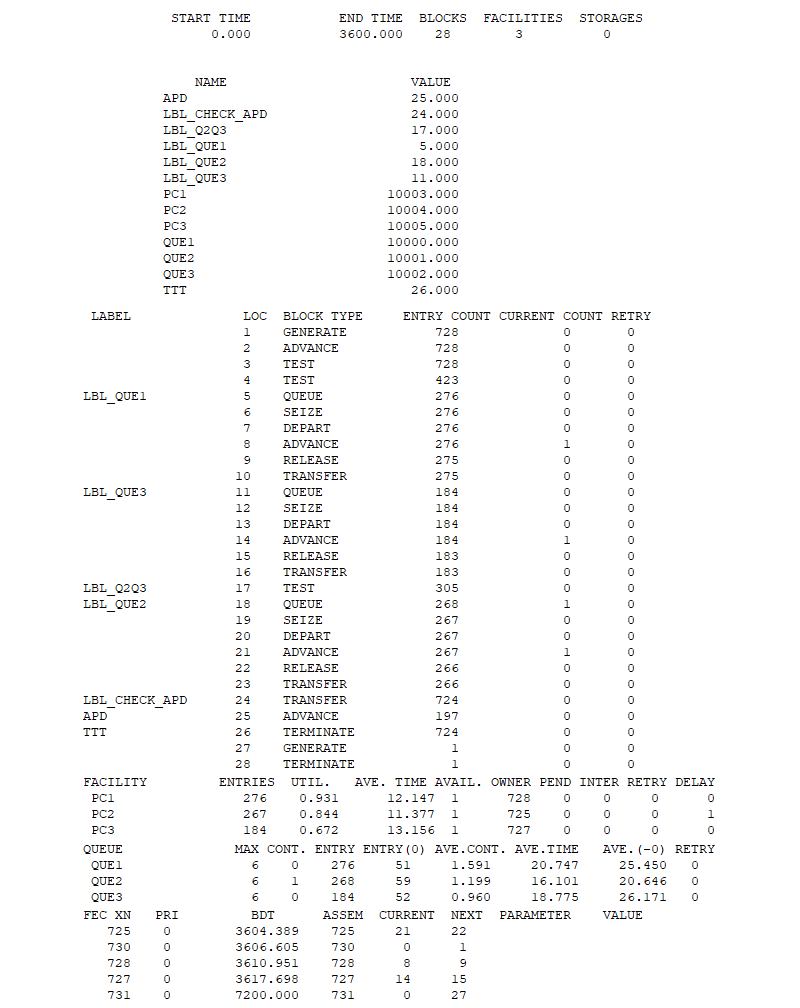
\includegraphics[width=\textwidth]{results_lab_6.png}
	\label{fig:results_lab_6}
	\caption{Результат работы программы.}
\end{figure}
